\subsection{QUOTIENT SPACE OF A SUBSPACE}

Let X be a topological space, A a subspace of X, R an equivalence relation on X, f the canonical map \(X \to X/R\) , g the restriction of f to A. The equivalence relation \(g(x) = g(y)\) on A is just the relation \(R_{A}\) induced by R on A (Set Theory R, § 5, no. 5). Let \(g = \psi \circ h \circ \varphi\) be the canonical decomposition of g, so that if j is the canonical injection of A into X we have a commutative diagram (*)

\begin{enumerate}
\def\labelenumi{(\Roman{enumi})}
\tightlist
\item
\end{enumerate}

\pandocbounded{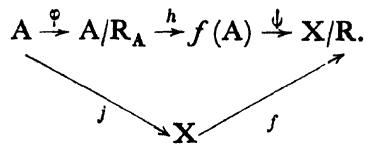
\includegraphics[keepaspectratio]{images/part001_6dc64900.jpg}}

PROPOSITION 10. The canonical bijection \(h: \mathbf{A} / \mathbf{R}_{\mathbf{A}} \to f(\mathbf{A})\) is continuous. Furthermore, the following three statements are equivalent:

\begin{enumerate}
\def\labelenumi{\alph{enumi})}
\item
  \(h\) is a homeomorphism.
\item
  Every open subset of A which is saturated with respect to \(R_{A}\) is the intersection with A of an open subset of X which is saturated with respect to R.
\item
  Every closed subset of A which is saturated with respect to \(R_{A}\) is the intersection with A of a closed subset of X which is saturated with respect to R.
\end{enumerate}

The first part of the proposition is immediate (no. 5). The second part follows from Proposition 8 of no. 5: if B is an open (resp. closed) subset of A which is saturated with respect to \(R_{A}\) , and \(g(B) = f(B)\) is the intersection with \(f(A)\) of an open (resp. closed) subset C of X/R, then B is the intersection with A of the open (resp. closed) subset \(\overline{f}(C)\)

of X, which is saturated with respect to R; and conversely, if B is the intersection with A of an open (resp. closed) subset D which is saturated with respect to R, then \(f(\mathbf{B})\) is the intersection of \(f(\mathbf{A})\) and \(f(\mathbf{D})\) , which is open (resp. closed) in X/R.

COROLLARY 1. If A is an open (resp. closed) subset of X which is saturated with respect to R, then the canonical mapping \(h: \mathrm{A}/\mathrm{R}_{\mathrm{A}} \rightarrow f(\mathrm{A})\) is a homeomorphism.

For if A is open (resp. closed) in X and saturated with respect to R, and if \(B \subset A\) is open (resp. closed) in A and saturated with respect to \(R_{A}\) , then B is open (resp. closed) in X and saturated with respect to R.

COROLLARY 2. If there is a continuous mapping \(u: \mathbf{X} \to \mathbf{A}\) such that \(u(x)\) is congruent to \(x \mod \mathbb{R}\) for each \(x \in \mathbf{X}\) , then \(f(\mathbf{A}) = \mathbf{X} / \mathbb{R}\) and the canonical mapping \(h: \mathbf{A} / \mathbb{R}_{\mathbf{A}} \to \mathbf{X} / \mathbb{R}\) is a homeomorphism.

Since each equivalence class mod R meets A, the canonical image of \(A/R_{A}\) in X/R is the whole of X/R; on the other hand, if U is open in A and is saturated with respect to \(R_{A}\) , it follows from the hypothesis that \(\overline{u}^{1}(U)\) is the set obtained by saturating U with respect to R; since u is continuous, \(\overline{u}^{1}(U)\) is open in X (§ 2, no. 1, Theorem 1). The corollary follows from this fact by virtue of Proposition 10.

Example. * Let R denote the equivalence relation \(x \equiv y \pmod{1}\) on the real line R (no. 4, Example) and let A denote the closed interval {[}0, 1{]}; A contains at least one point of each equivalence class mod R. The canonical mapping of \(\mathrm{A} / \mathbb{R}_{\mathbf{A}}\) onto the torus T is a homeomorphism; for if F is closed in A (and hence in R), in order to saturate F with respect to the relation R we have to take the union of the closed sets \(\mathrm{F} + n\) (for all \(n \in \mathbf{Z}\) ), which evidently form a locally finite family, so that their union is closed (§ 1, no. 5, Proposition 4); the assertion follows from this. We remark that \(\mathrm{A} / \mathbb{R}_{\mathbf{A}}\) is obtained by identifying the points 0 and 1 in A. *

